\section{Results}
\subsection{Descriptive CGPA patterns}
Three questionnaire variables show the clearest corrected association with CGPA: desired-department match ($\rho=+0.119$, adjusted $q=0.0010$), attendance ($\rho=+0.090$, $q=0.0197$), and outside commitments ($\rho=-0.086$, $q=0.0202$). Each association is small. Figures~\ref{fig:attendance-cgpa}--\ref{fig:department-cgpa} show group composition rather than causal effects.

\begin{figure}[H]\centering
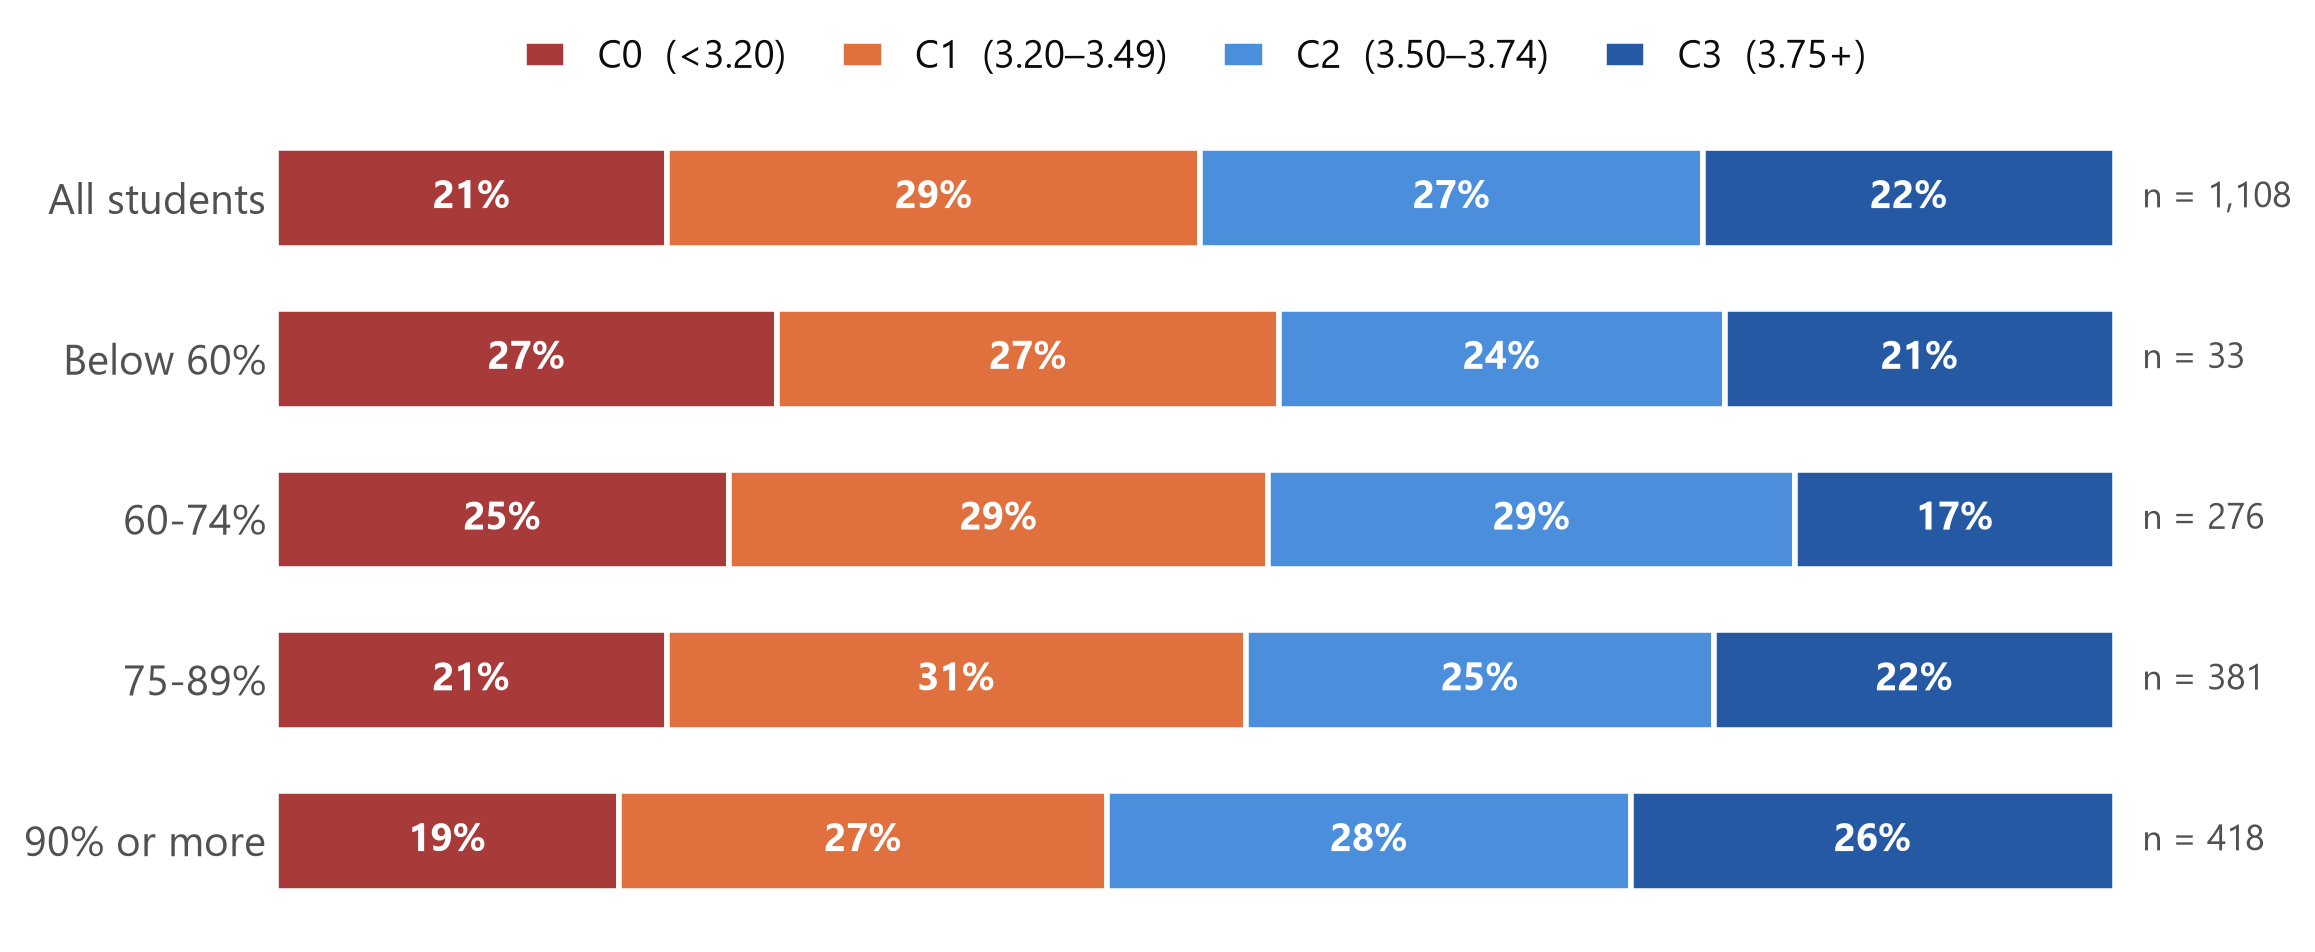
\includegraphics[width=0.9\textwidth]{figures/attendance_cgpa.png}
\caption{CGPA-group composition by attendance band. Students reporting 90\% or more attendance have a 55\% C2/C3 share, compared with 46\% for the 60--74\% group.}
\label{fig:attendance-cgpa}
\end{figure}

\begin{figure}[H]\centering
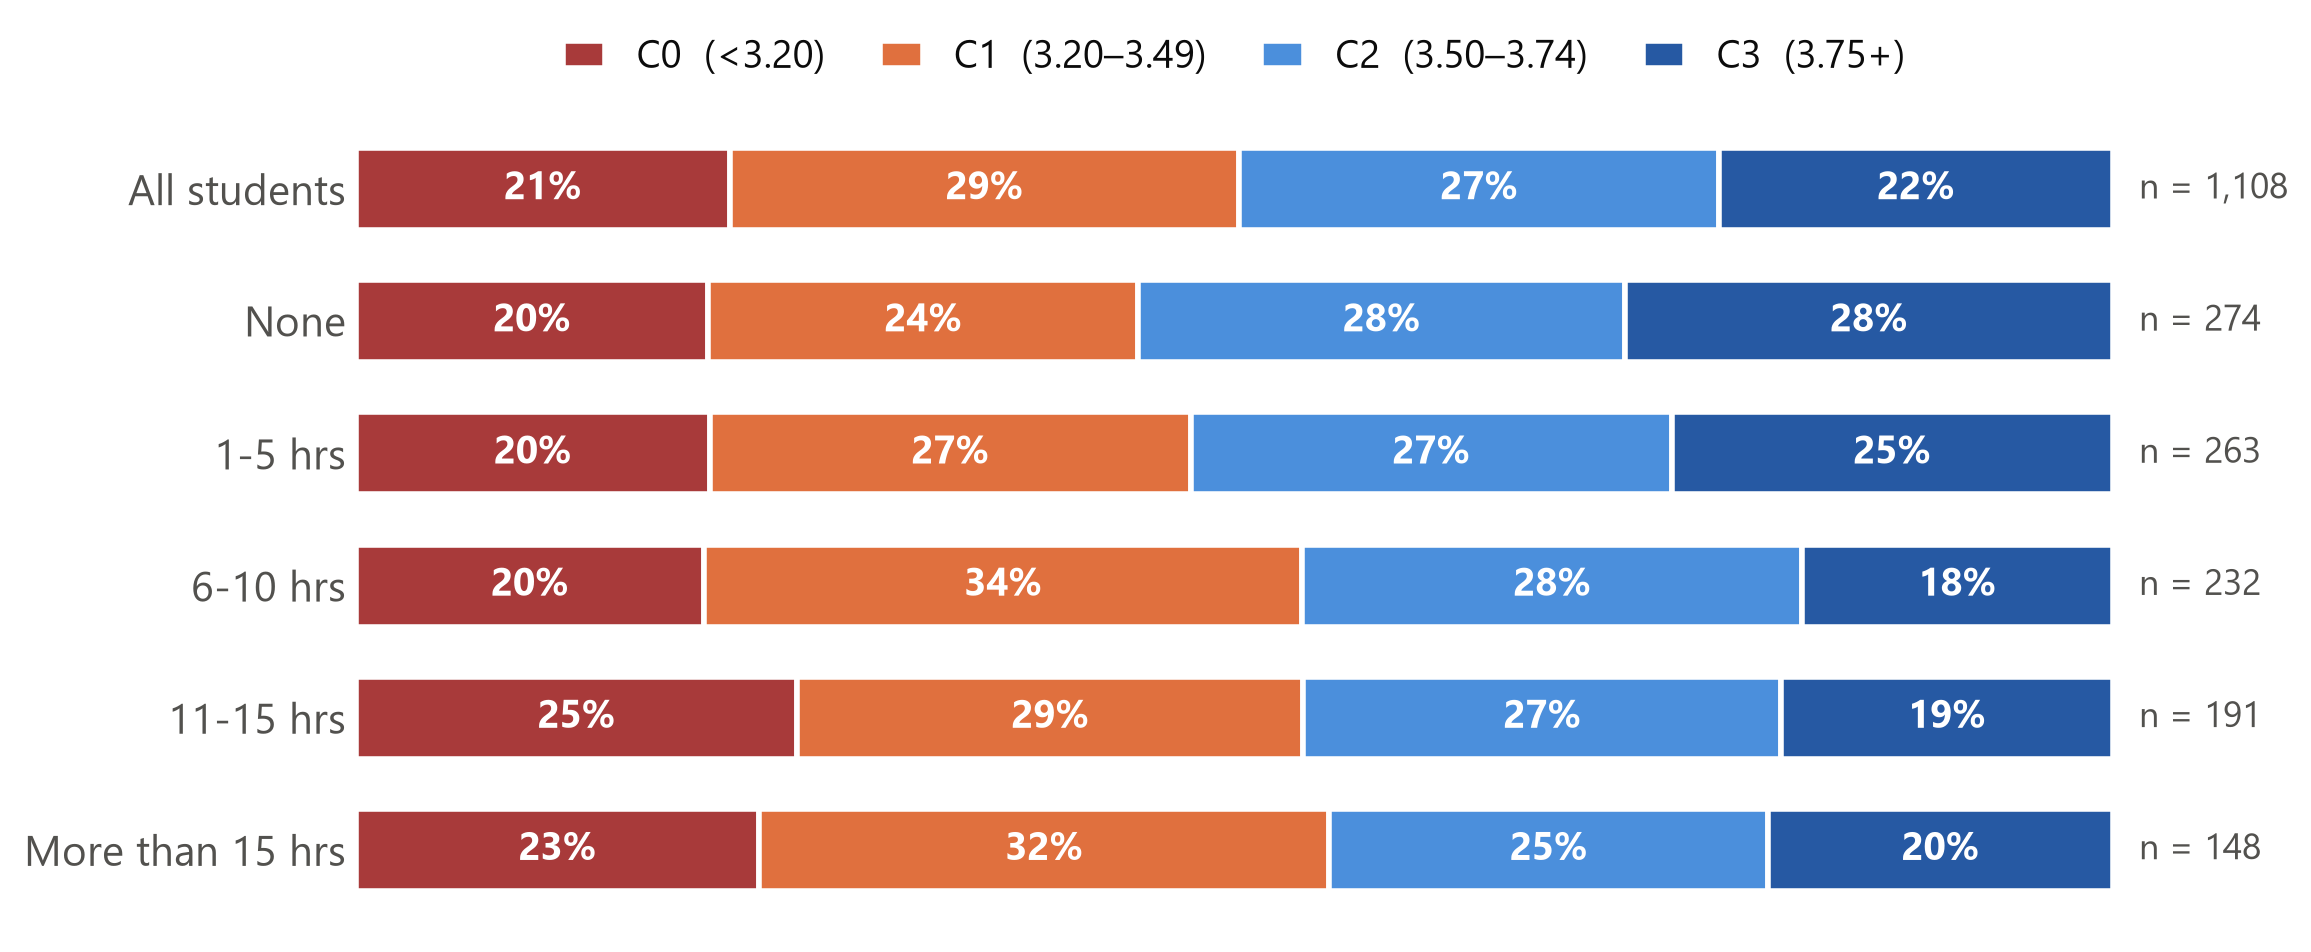
\includegraphics[width=0.9\textwidth]{figures/commitments_cgpa.png}
\caption{CGPA-group composition by weekly outside commitments. The C2/C3 share is 56\% for no outside commitments and 45\% above 15 hours.}
\label{fig:commitments-cgpa}
\end{figure}

\begin{figure}[H]\centering
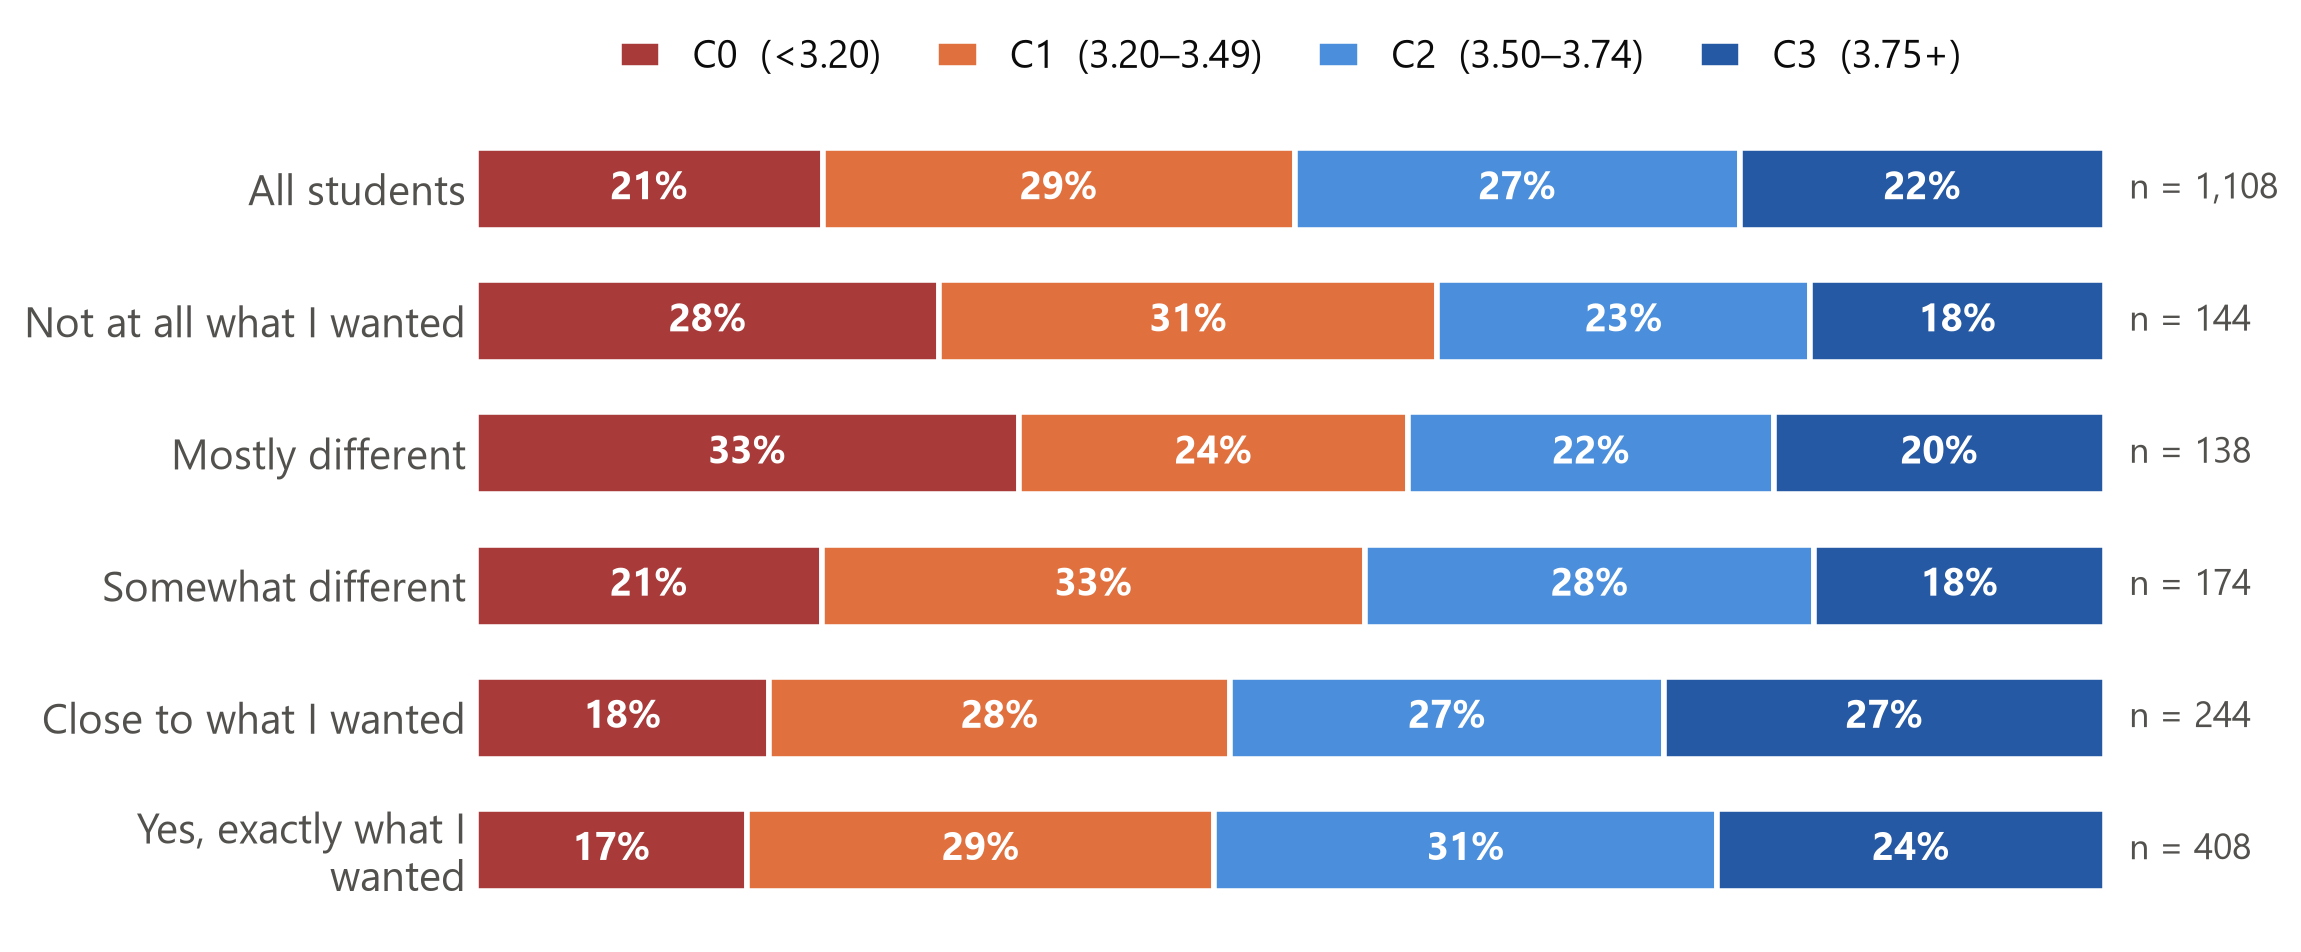
\includegraphics[width=0.9\textwidth]{figures/department_cgpa.png}
\caption{CGPA-group composition by desired-department match. The C2/C3 share is 55\% among students who report exactly the department they wanted and 41\% among those reporting no match.}
\label{fig:department-cgpa}
\end{figure}

\subsection{WEKA 10-fold cross-validation}
Table~\ref{tab:weka-cv} reports the final like-for-like model comparison on all 1,102 eligible records. J48 is the strongest SGPA model at 30.13\%, only 3.27 percentage points above ZeroR. Naive Bayes is strongest for questionnaire-only CGPA at 30.04\%, 1.00 point above ZeroR. Random Forest is strongest for the main CGPA task at 43.92\%, 14.88 points above ZeroR. These results show weak prediction from questionnaire answers alone and a clearer predictive contribution from recent SGPA.

\begin{table}[H]\centering
\caption{WEKA stratified 10-fold cross-validation accuracy on 1,102 records, seed 1.}\label{tab:weka-cv}
\begin{tabular}{lrrr}\toprule
Model&Recent SGPA (\%)&Questionnaire CGPA (\%)&Main CGPA (\%)\\\midrule
J48&30.13&26.68&38.29\\
Random Forest&29.76&29.40&\textbf{43.92}\\
SMO&25.95&27.86&37.11\\
Logistic&24.95&29.58&36.84\\
Naive Bayes&26.68&\textbf{30.04}&38.11\\
ZeroR&26.86&29.04&29.04\\\bottomrule
\end{tabular}
\end{table}

\begin{figure}[H]\centering
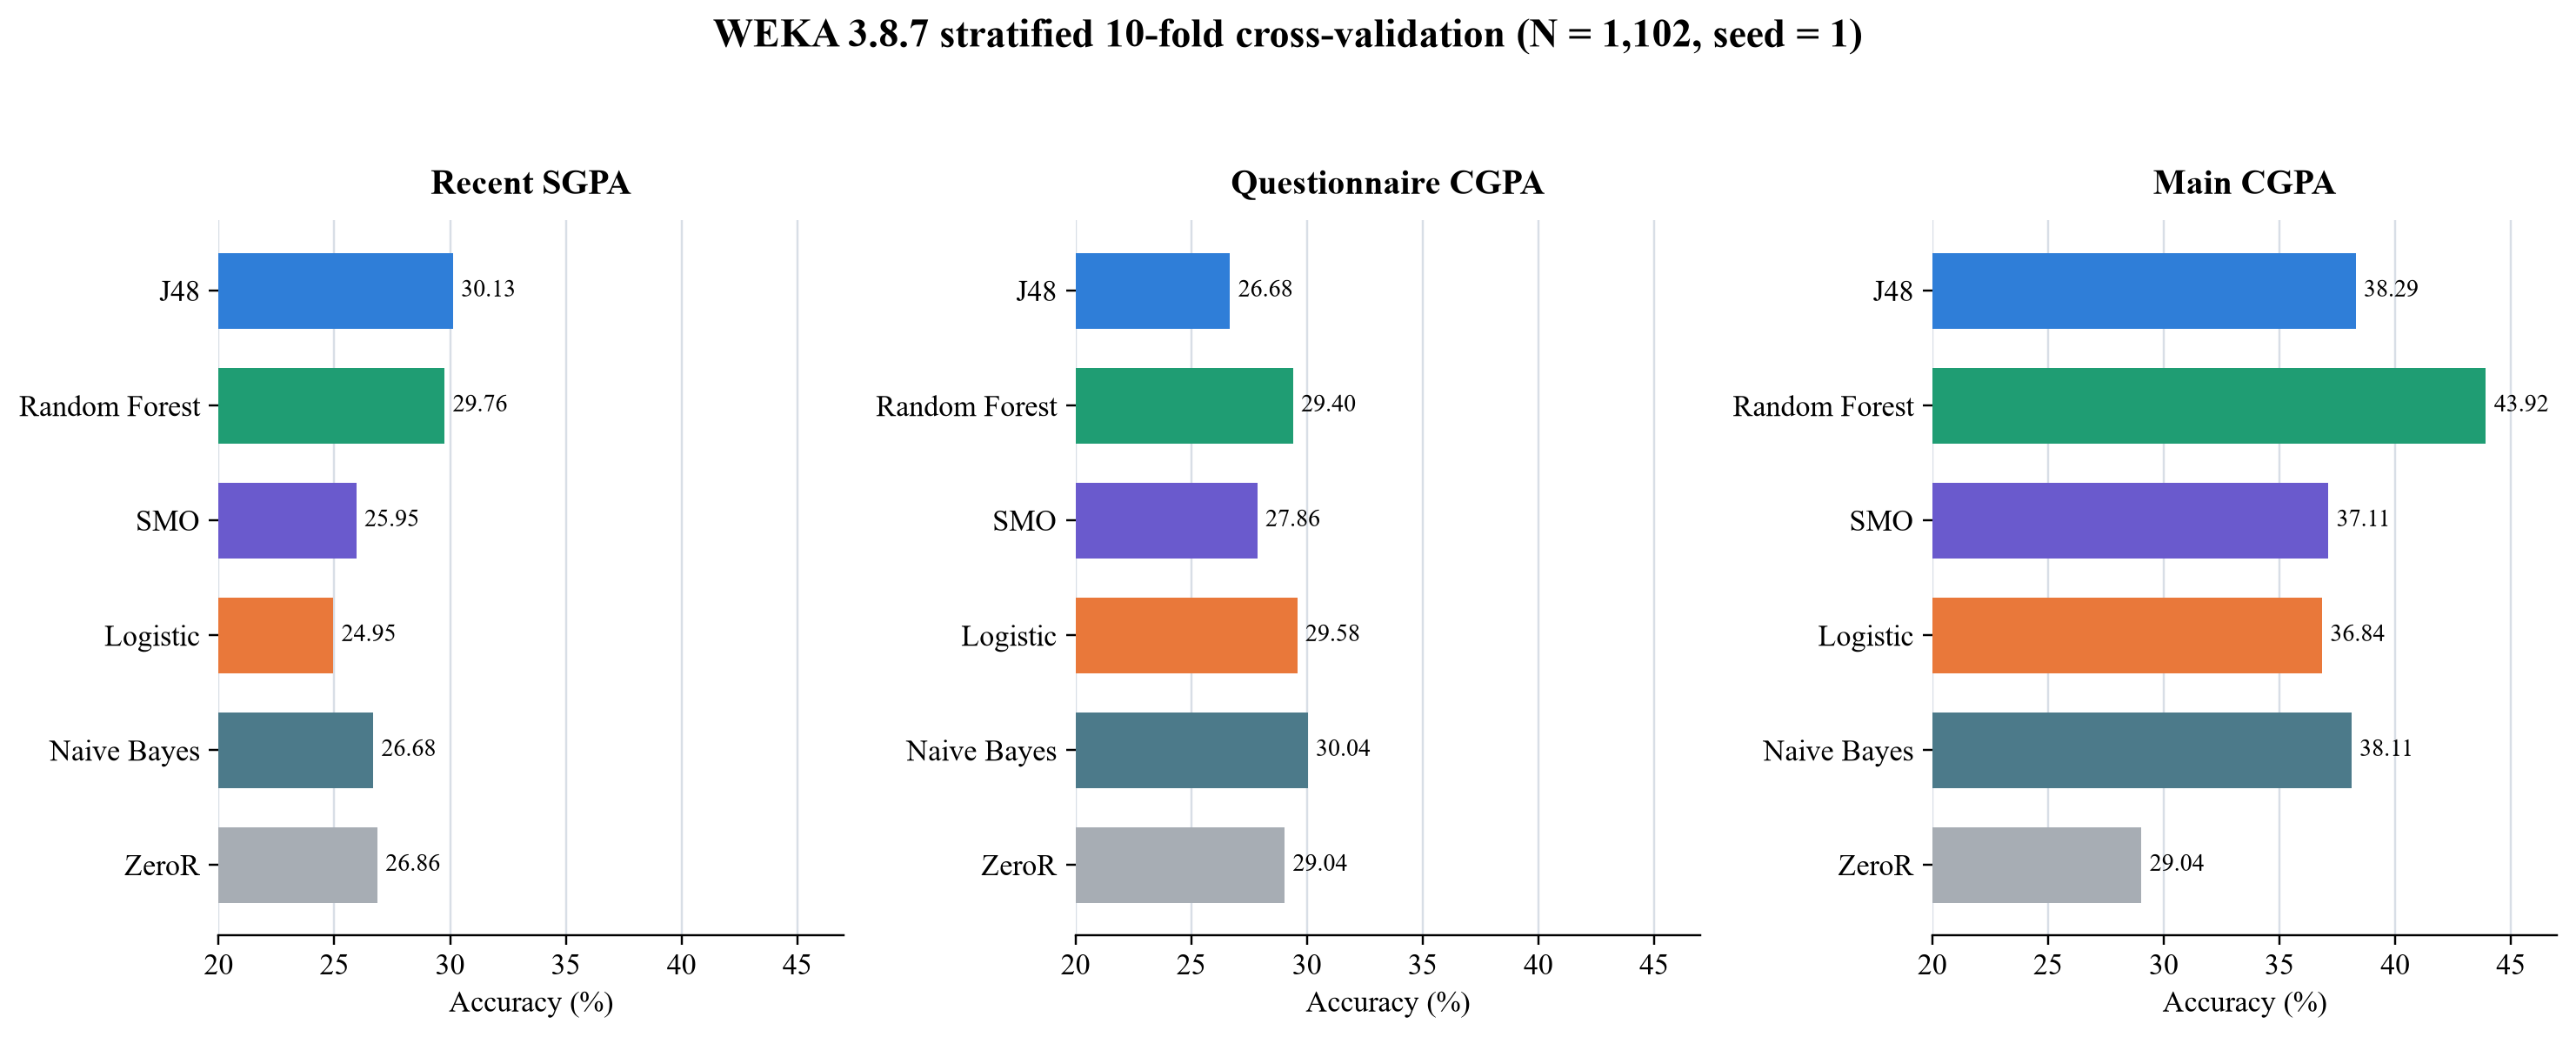
\includegraphics[width=0.96\textwidth]{figures/weka_accuracy_comparison.png}
\caption{The final WEKA cross-validation comparison. Each group uses the same 1,102 eligible students and evaluation seed.}
\label{fig:weka-accuracy}
\end{figure}

\subsection{Readable WEKA J48 trees on the fixed split}
The fixed-split J48 runs use the same 881 training and 221 test rows with \code{-C 0.25 -M 40}. The larger leaf requirement produces compact trees that can be shown without redrawing them. Table~\ref{tab:weka-holdout} reports each tree against the ZeroR test baseline.

\begin{table}[H]\centering
\caption{Fixed-split WEKA J48 results.}\label{tab:weka-holdout}
\begin{tabular}{lrrrr}\toprule
Prediction&Train (\%)&Test (\%)&Baseline (\%)&Change (pp)\\\midrule
Recent SGPA&39.39&29.86&27.15&+2.71\\
Questionnaire CGPA&36.55&32.13&28.96&+3.17\\
Main CGPA&46.20&49.77&28.96&+20.81\\\bottomrule
\end{tabular}
\end{table}

The SGPA tree begins with routine manageability and creates 13 leaves. Its 29.86\% test accuracy remains close to the 27.15\% baseline, so its branches are exploratory. Figure~\ref{fig:weka-sgpa-tree} is the actual WEKA TreeVisualizer export from this run.

\begin{figure}[H]\centering
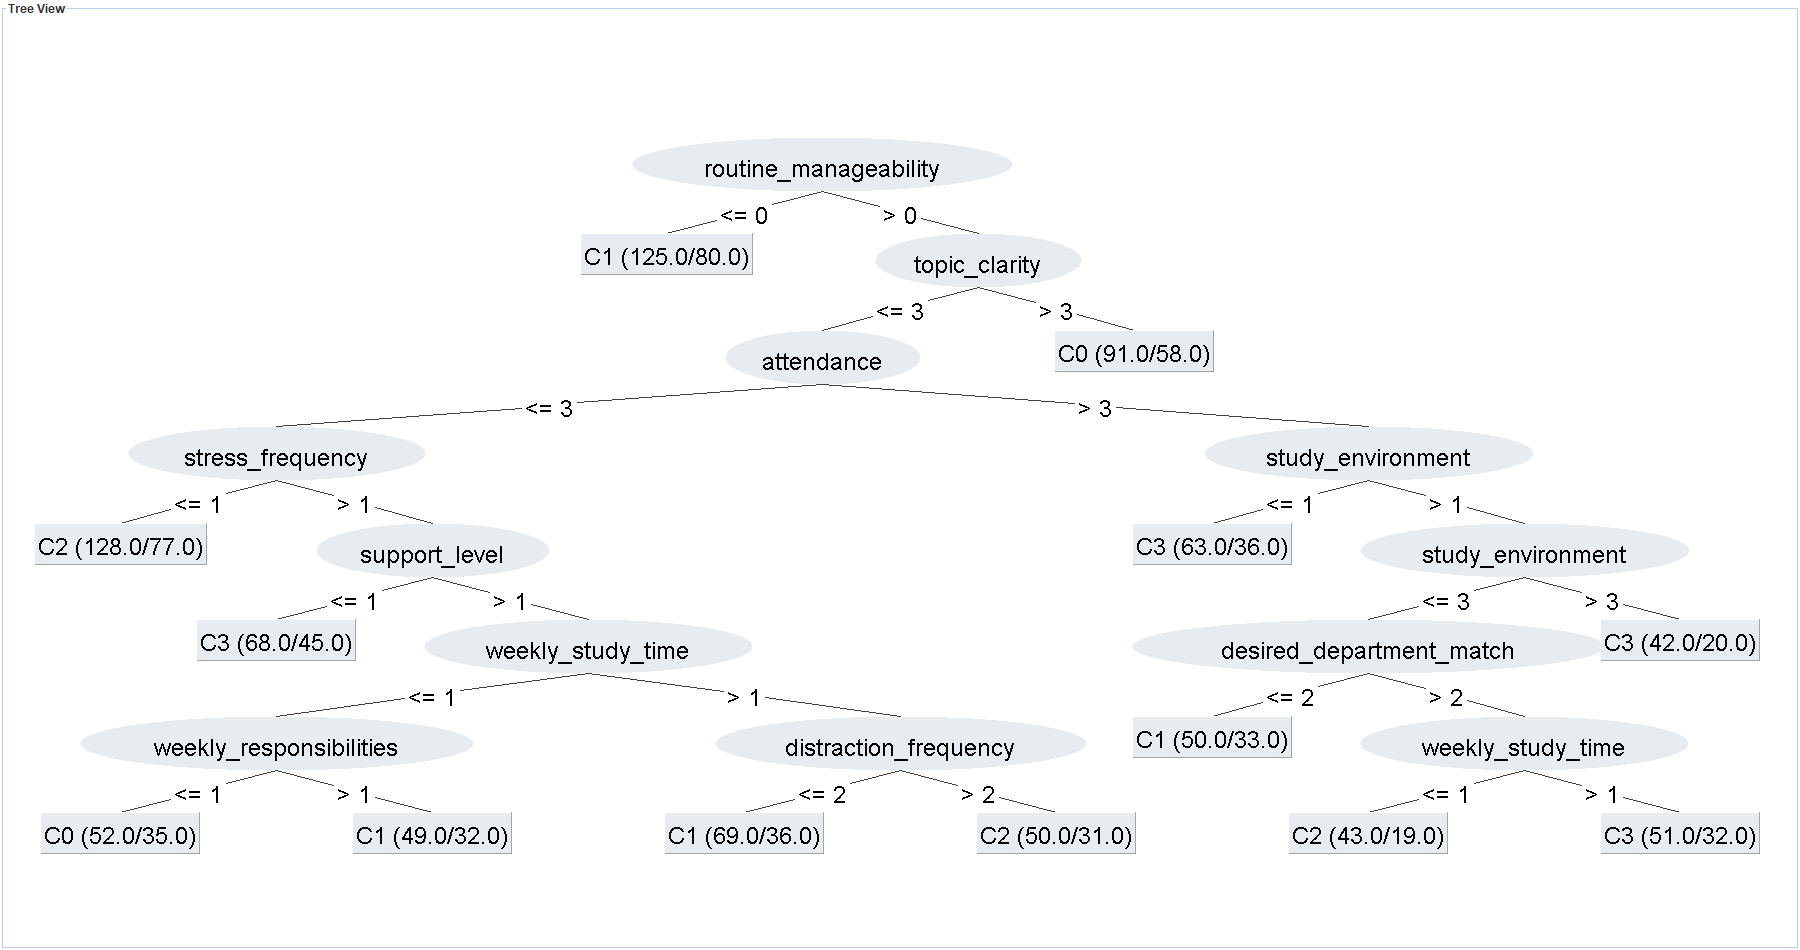
\includegraphics[width=\textwidth,height=0.70\textheight,keepaspectratio]{figures/weka_sgpa_tree.png}
\caption{Actual WEKA J48 tree for recent SGPA from the 12 questionnaire inputs.}
\label{fig:weka-sgpa-tree}
\end{figure}

The questionnaire-only CGPA tree reaches 32.13\% on the fixed test set, 3.17 points above its baseline, but the 10-fold model comparison remains near baseline. Figure~\ref{fig:weka-questionnaire-tree} shows why the result should be treated cautiously: the tree uses several survey variables while the four classes remain mixed.

\begin{figure}[H]\centering
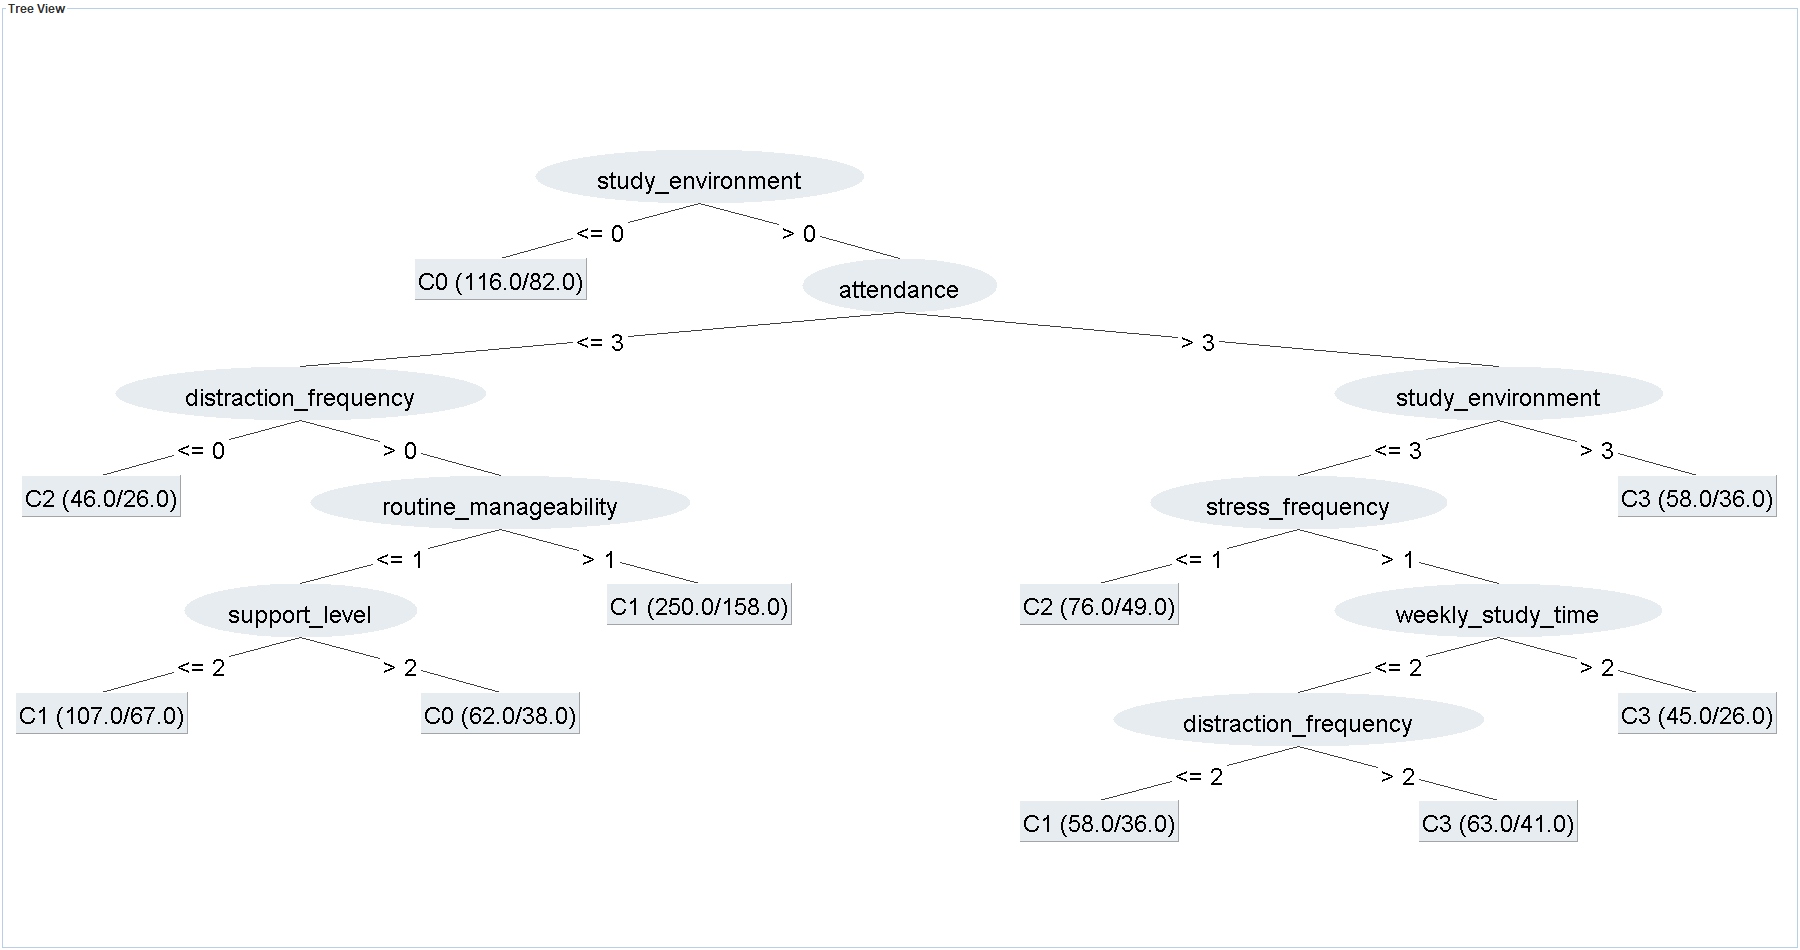
\includegraphics[width=\textwidth,height=0.70\textheight,keepaspectratio]{figures/weka_questionnaire_tree.png}
\caption{Actual WEKA J48 tree for CGPA using only the 12 questionnaire inputs.}
\label{fig:weka-questionnaire-tree}
\end{figure}

The main CGPA tree starts with recent SGPA. For students in the highest recent-SGPA band, outside commitments and desired-department match provide the remaining splits. The resulting six-leaf tree reaches 49.77\% on the fixed test set. This single-split result complements the more stable 10-fold Random Forest result; it does not replace it.

\begin{figure}[H]\centering
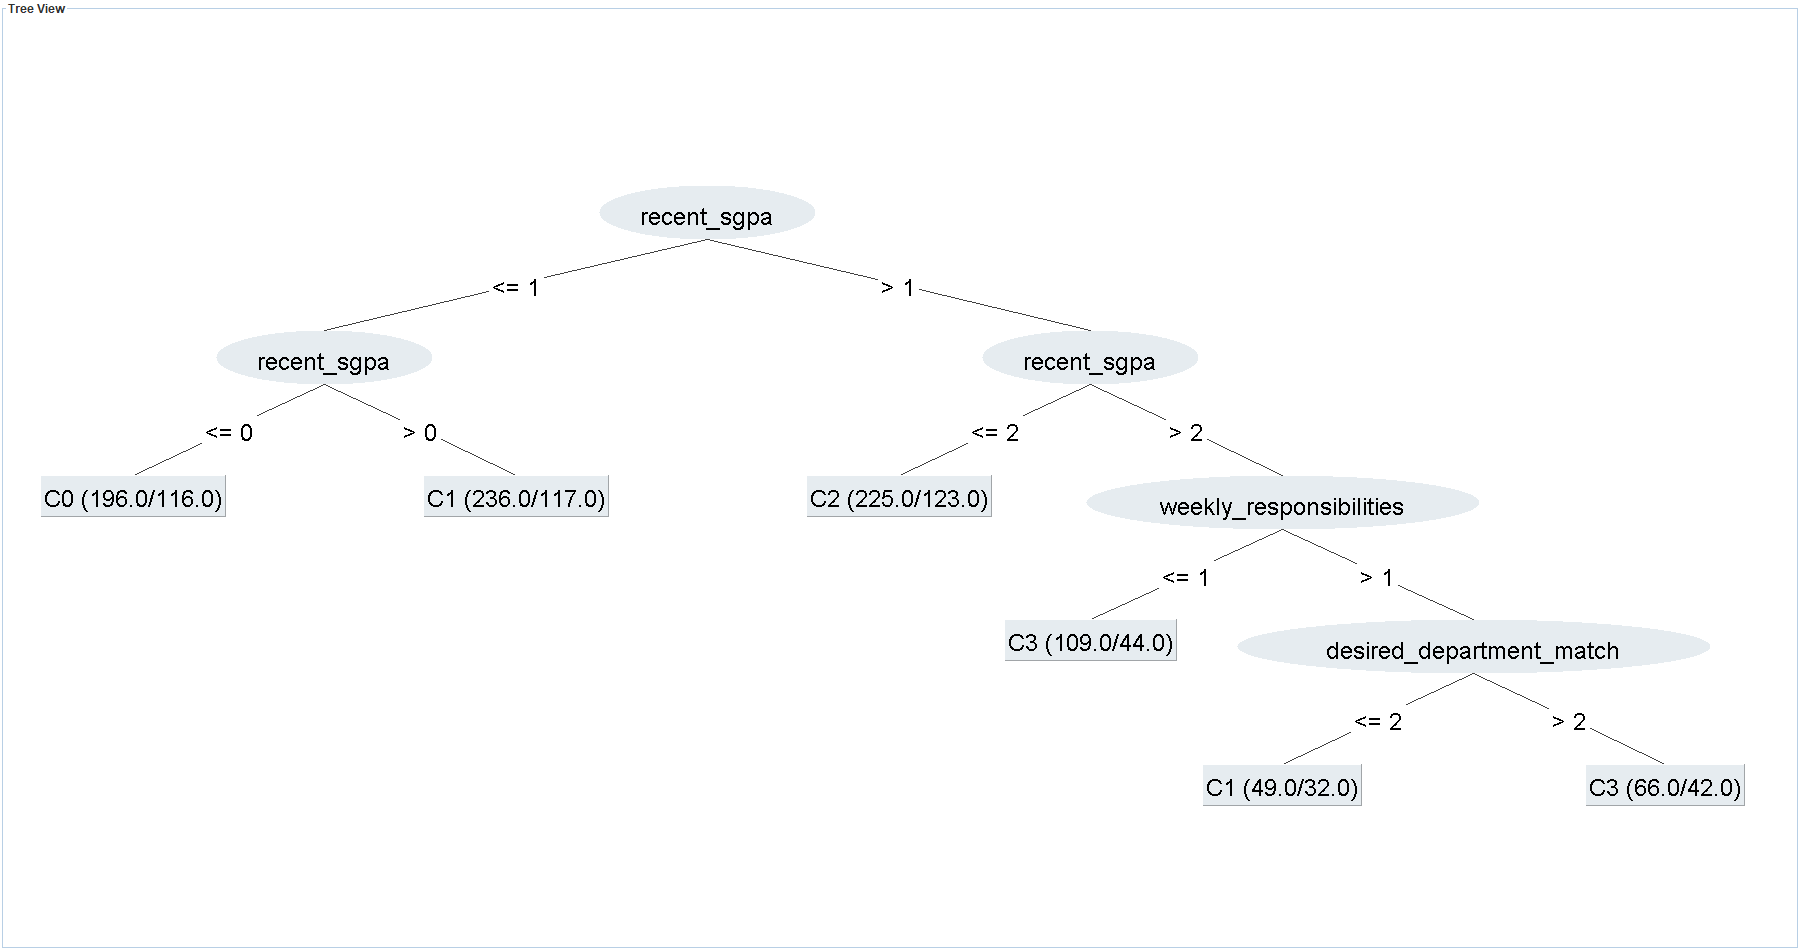
\includegraphics[width=\textwidth,height=0.65\textheight,keepaspectratio]{figures/weka_main_tree.png}
\caption{Actual WEKA J48 tree for the main CGPA task. Recent SGPA forms the first split.}
\label{fig:weka-main-tree}
\end{figure}

\subsection{Main-tree confusion matrix and ordered errors}
The main J48 tree correctly classifies 110 of 221 test students. Rows in Figure~\ref{fig:weka-main-confusion} are actual groups and columns are predicted groups. Seventy errors are one adjacent band away and 41 are two or three bands away.

\begin{figure}[H]\centering
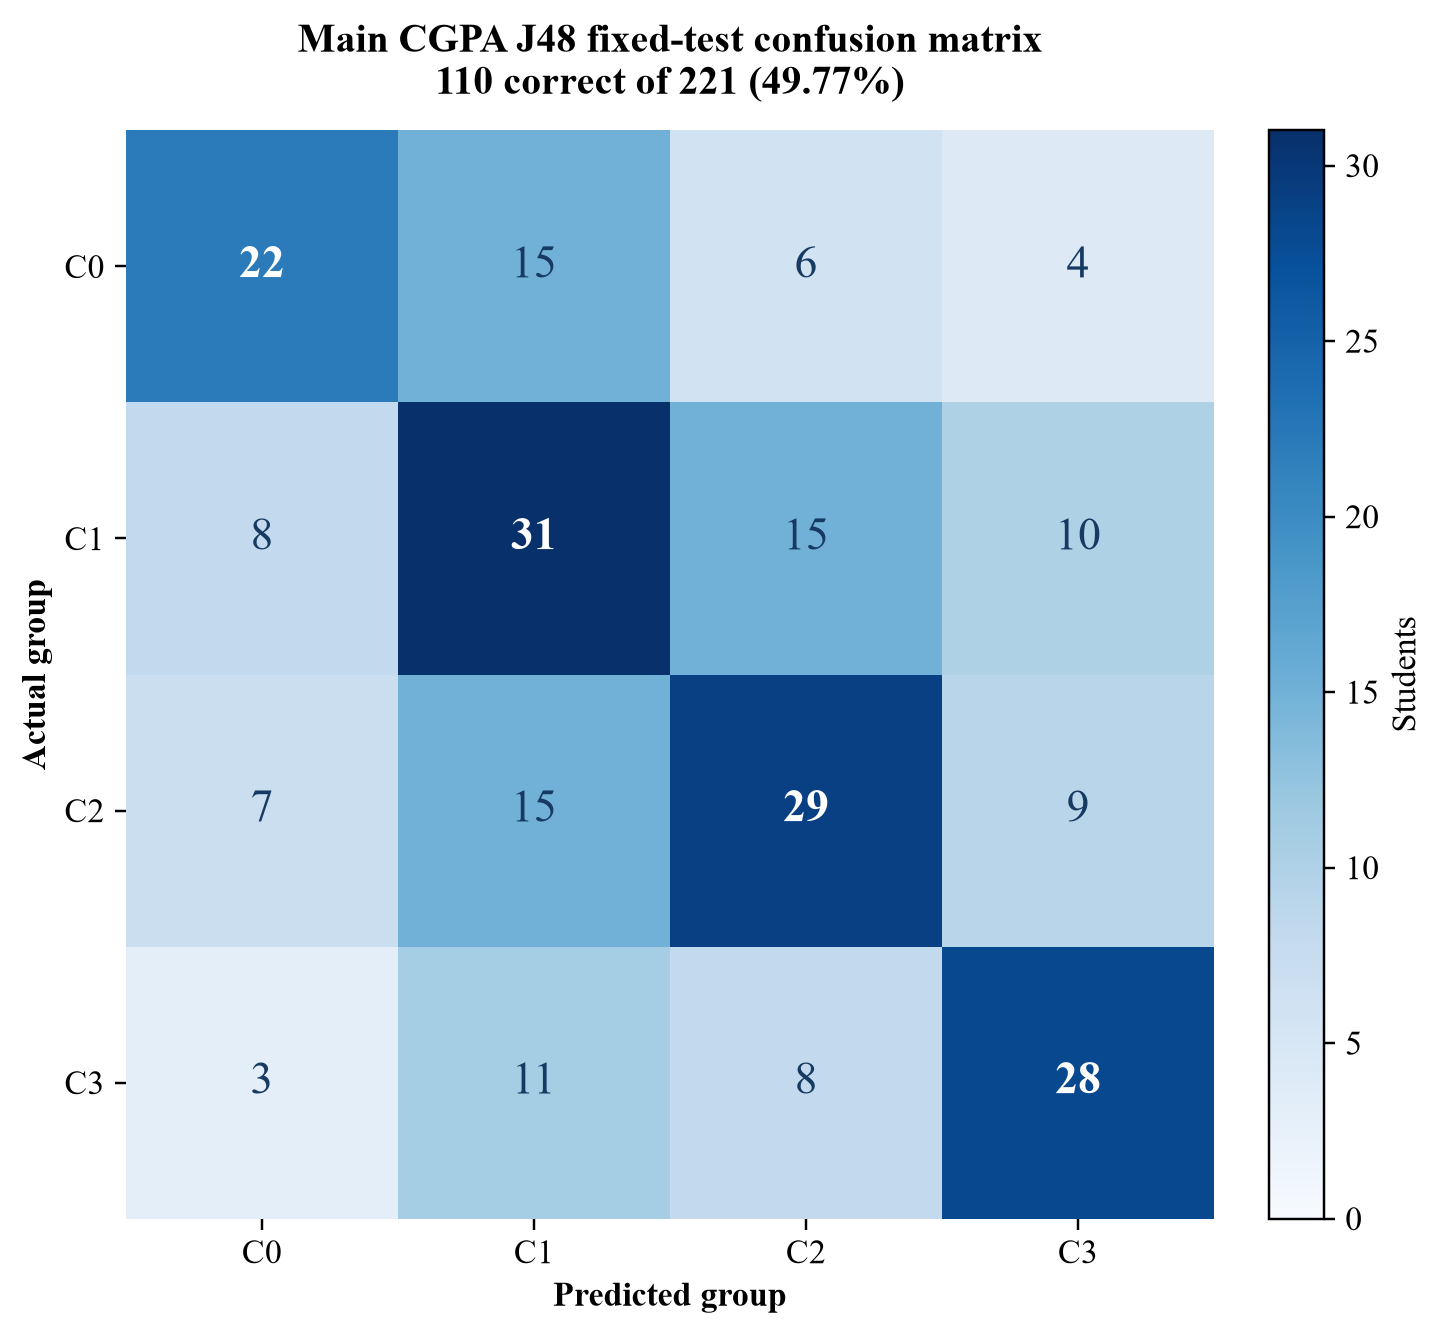
\includegraphics[width=0.78\textwidth]{figures/weka_main_confusion_matrix.png}
\caption{Fixed-test confusion matrix for the main WEKA J48 tree.}
\label{fig:weka-main-confusion}
\end{figure}

\begin{table}[H]\centering
\caption{Ordered error distribution for the 221-student fixed test set.}\label{tab:ordinal-errors}
\begin{tabular}{lrr}\toprule Absolute class distance&Students&Share (\%)\\\midrule
0: exact group&110&49.77\\
1: adjacent group&70&31.67\\
2 or 3: farther group&41&18.55\\\midrule
Mean absolute class distance&\multicolumn{2}{c}{0.719 groups}\\\bottomrule
\end{tabular}
\end{table}

\subsection{WEKA output evidence}
The repository stores the raw text log, serialized model, textual tree, DOT graph, TreeVisualizer image, and rendered output capture for each J48 target. Figure~\ref{fig:weka-output} shows the main-task output generated from the final WEKA 3.8.7 log.

\begin{figure}[H]\centering
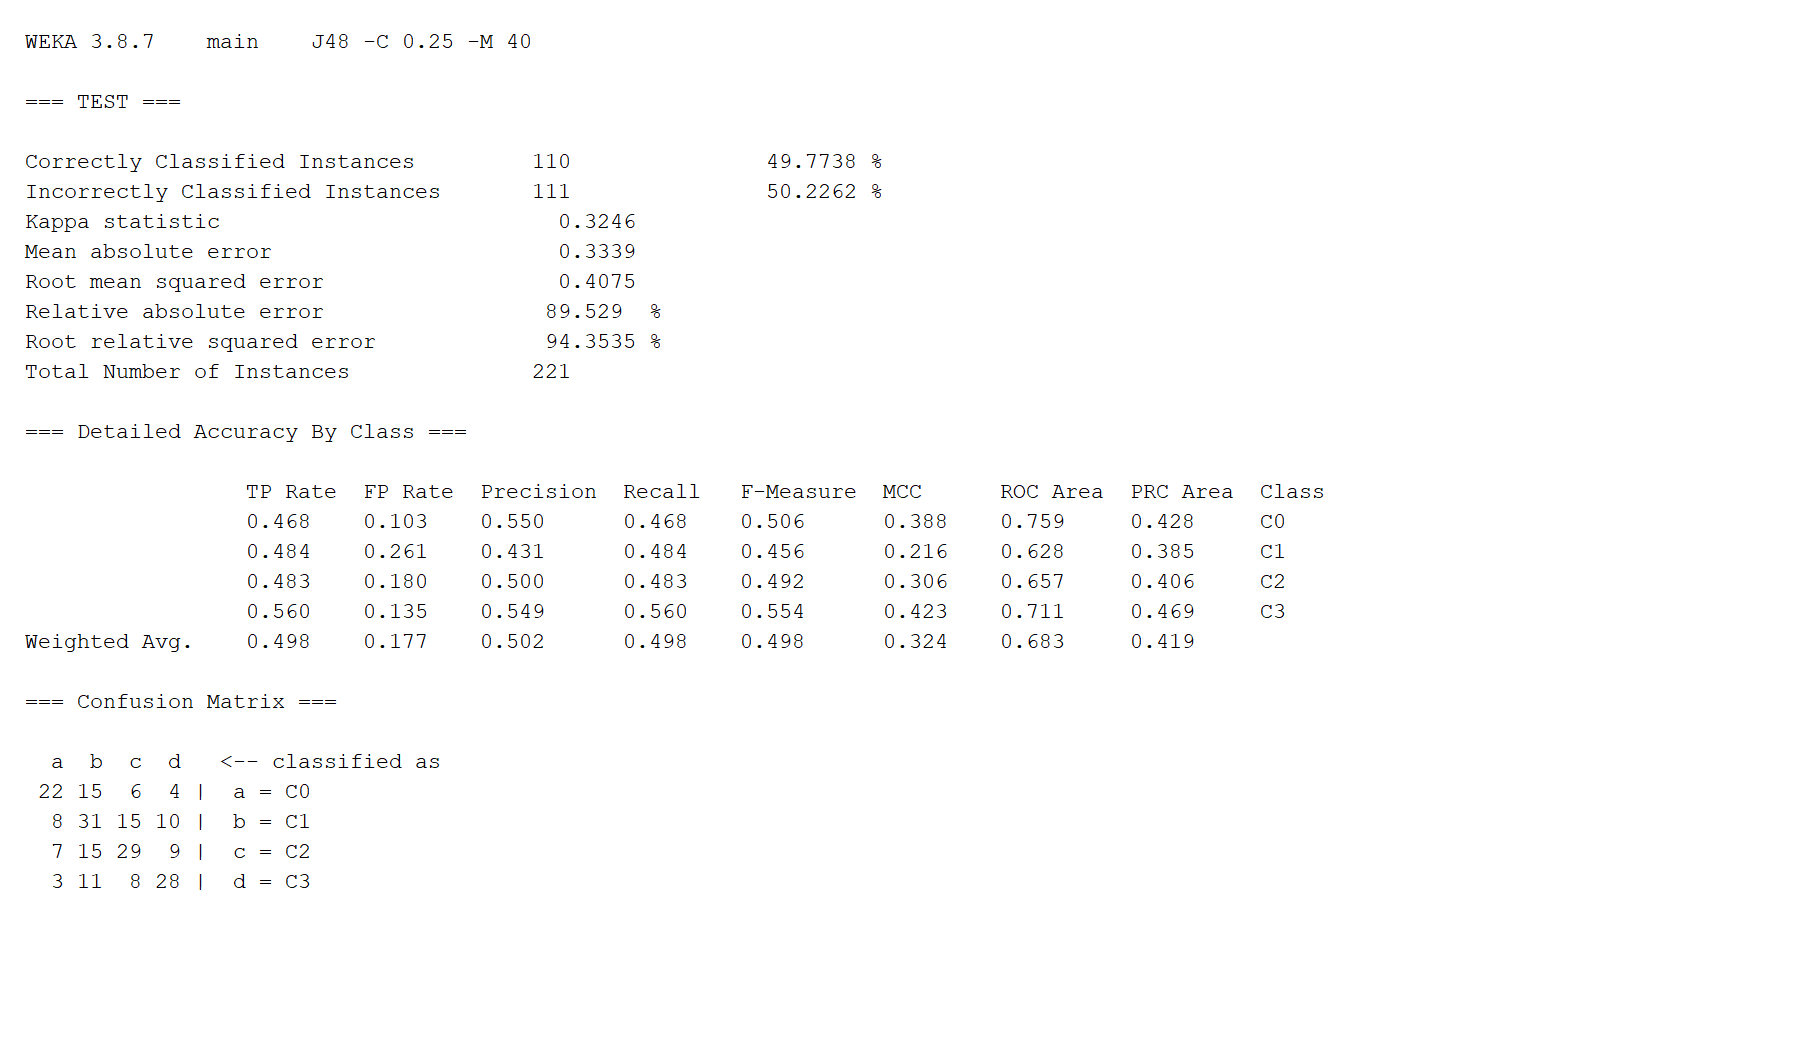
\includegraphics[width=\textwidth,height=0.72\textheight,keepaspectratio]{figures/weka_main_output.png}
\caption{Rendered WEKA output for the main CGPA J48 run, including settings, accuracy, and confusion matrix.}
\label{fig:weka-output}
\end{figure}

\subsection{Comparison with previous studies}
\begin{table}[H]\centering\scriptsize
\caption{Related-work comparison. Accuracy values use different data and targets and are not directly comparable.}\label{tab:related}
\begin{tabularx}{\textwidth}{p{0.16\textwidth}p{0.20\textwidth}p{0.23\textwidth}Y}\toprule
Study&Population or target&Models&Reported result and relation\\\midrule
Ahmed (2024) \cite{ahmed2024}&Student-performance classification&K-means, SVM, Decision Tree, Naive Bayes, KNN&SVM reported 96\% after tuning. The current work emphasises a merged engineering survey and target-specific validation.\\
Maruf et al. (2024) \cite{maruf2024}&Bangladeshi SSC and HSC results&Tuned models, stacking, SHAP&Stacking reported 82.23\% for SSC and 86.89\% for HSC. The target and population differ from four-band university CGPA.\\
Albonny and Duru (2026) \cite{albonny2026}&More than 8,000 secondary-school students; course-grade regression&Linear Regression, Decision Tree, Random Forest, DNN&Random Forest reported $R^2=93.3$. The current project uses ordinal classification and university survey data.\\
This project&1,102 eligible engineering students; CGPA C0--C3&WEKA J48, Random Forest, SMO, Logistic, Naive Bayes, ZeroR&Random Forest reaches 43.92\% under 10-fold validation; the readable J48 reaches 49.77\% on one fixed 221-row test set.\\\bottomrule
\end{tabularx}
\end{table}
